\chapter{Precauciones}\label{ch:precautions}

Este capítulo reúne las normas de seguridad obligatorias que acompañan a cada cuadro de instrumentos \ReplicaGenOne{} y \ReplicaNextLong{}. Ignorar cualquiera de estos puntos es la forma más rápida de dañar la electrónica u obtener lecturas poco fiables.

\begin{enumerate}
    \item \textbf{Desconecte la batería del vehículo antes de comenzar la instalación.} Trabajar con el mazo energizado puede parecer más rápido, pero ya se han destruido varios tableros por cortocircuitos provocados por un arnés con tensión.
    \item \textbf{No alimente nunca las entradas de sensores con una fuente de tensión externa.} Los canales de temperatura del refrigerante, temperatura del aceite, temperatura exterior y nivel de combustible están diseñados únicamente para sensores pasivos. Incluso una prueba “inofensiva” a través de una resistencia quema la circuitería de medida.
    \item \textbf{Recuerde que los paneles de las generaciones~1 y~1.5 no tienen fusible interno.} El primer elemento de protección es el fusible de 15~A de la caja de fusibles de Volkswagen. Reacciona demasiado tarde para salvar el cuadro ante errores de cableado.
    \item \textbf{Proteja la unidad de la luz solar directa.} La exposición prolongada lava los segmentos LCD y reduce permanentemente el contraste.
    \item \textbf{No intente forzar la retroiluminación LED.} Las generaciones~1, 1.5 y~2 emplean iluminación de corriente fija. Si la imagen diurna es tenue, añada sombra alrededor de la visera en lugar de aumentar la corriente de alimentación.
    \item \textbf{Atención a las resonancias en velocímetros accionados por cable.} Los accionamientos mecánicos suelen oscilar entre 40 y 60~km/h. Instale el sensor electrónico suministrado---se incluye con todos los kits Gen~1.5 y Gen~2 actuales---siempre que sea posible.
    \item \textbf{Planifique controles externos de MFA para los tableros de la Generación~2.} Se eliminó el sensor táctil con el logotipo de VW, por lo que el cambio de modo MFA debe provenir de la palanca de la columna de dirección o de otro interruptor externo.
    \item \textbf{Tenga en cuenta la corriente de reposo.} Un cuadro de la Generación~2 consume aproximadamente 11--13~mA de la batería del vehículo incluso cuando el encendido está apagado. Este consumo en reposo no se puede reducir.
    \item \textbf{El consumo instantáneo de combustible no viene instalado de fábrica.} La función puede añadirse a las unidades Gen~1 y Gen~1.5 siguiendo las instrucciones indicadas a continuación, pero no se ha validado para el hardware Gen~2.
        \displayurl{https://www.youtube.com/watch?v=qWqvYc9388U}
\end{enumerate}

\begin{figure}[htbp]
    \centering
    \begin{subfigure}{0.46\textwidth}
        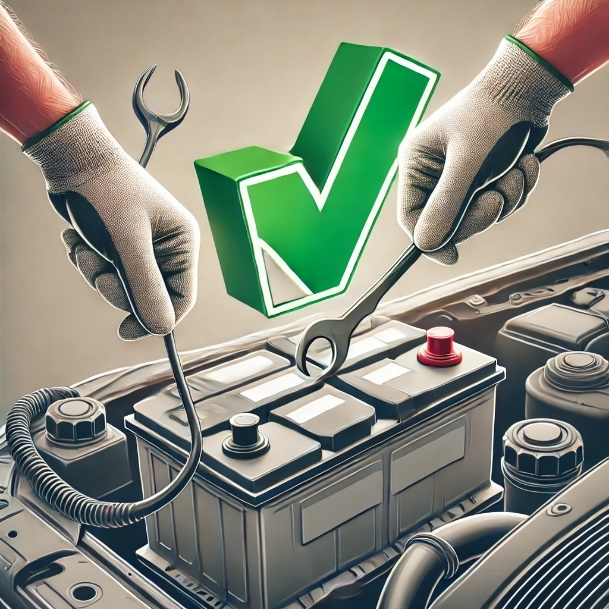
\includegraphics[width=\linewidth]{digifiz_manual/image001.jpg}
        \caption{Etiqueta que recalca la desconexión de la batería durante la instalación.}
    \end{subfigure}\hfill
    \begin{subfigure}{0.46\textwidth}
        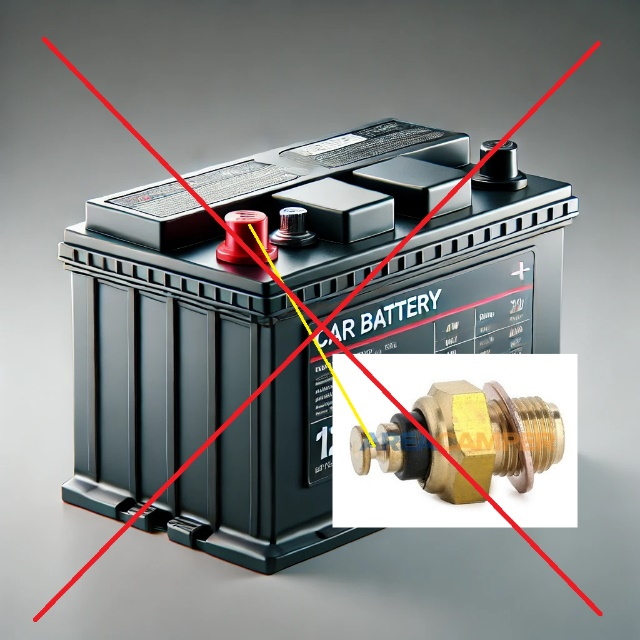
\includegraphics[width=\linewidth]{digifiz_manual/image002.jpg}
        \caption{Aviso incluido con el arnés de sensores contra la tensión externa.}
    \end{subfigure}
    \caption{Carteles de seguridad suministrados con el kit de cableado.}
\end{figure}
